
% This LaTeX was auto-generated from MATLAB code.
% To make changes, update the MATLAB code and republish this document.

\documentclass{article}
\usepackage{graphicx}
\usepackage{color}

\sloppy
\definecolor{lightgray}{gray}{0.5}
\setlength{\parindent}{0pt}

\begin{document}

    
    
\section*{Connor McGarty, cmcgarty - HW01: P1.9 from Chapra Text}

\begin{par}
File: cmcgarty\_EE254\_HW01\_P1\_9.m
\end{par} \vspace{1em}
\begin{par}
Submission Date: Tuesday, January 28, 2020 - 1/28/20
\end{par} \vspace{1em}
\begin{par}
Problem, P1.9: A storage tank contains a liquid at depth $y$ where $y = 0$ when the tank is half full. Liquid is withdrawn at a constant flow rate $Q$ to meet demands. The contents are resupplied at a sinusoidal rate $3Q\sin^{2}(t)$. Equation (1.14) can be written for this system as:
\end{par} \vspace{1em}
\begin{par}
$$\frac{d(Ay)}{dt} = 3Q\sin^{2}(t)$$
\end{par} \vspace{1em}
\begin{par}
or,
\end{par} \vspace{1em}
\begin{par}
change in volume = inflow - outflow
\end{par} \vspace{1em}
\begin{par}
Or, since the surface area A is constant:
\end{par} \vspace{1em}
\begin{par}
$$\frac{dy}{dt} = 3*\frac{Q}{A}*\sin^{2}(t) - \frac{Q}{A}$$
\end{par} \vspace{1em}
\begin{par}
Use Euler's method to solve for the depth $y$ from $t=0$ to $10s$ with a step size of 0.5 s. The parameter values are $A = 1250 m^{2}$ and $Q = 450 \frac{m^{3}}{s}$ . Assume that the initial condition is $y = 0$ .
\end{par} \vspace{1em}

\subsection*{Contents}

\begin{itemize}
\setlength{\itemsep}{-1ex}
   \item Solution
\end{itemize}


\subsection*{Solution}

\begin{verbatim}
clear;clc;
% Inital conditions
half_full = 0; % m
surface_area = 1250; % m^2, variable A
outflow_rate = 450; % m^3/d, variable Q

% set time conditions
t_start = 0; % s
t_stop = 10; % s
t_current = t_start;
t_previous = t_current;
t_delta = 0.5; % s
t_vector = []; % s
t_vector(1) = t_start;

y_init = 0; % m
y_vector = []; % m
y_vector(1) = y_init;
y_current = y_init;
y_previous = y_current;

iterator = 1;
done = false; % loop flag

while (done == false)
    iterator = iterator + 1;
    slope = 3 .* (outflow_rate ./ surface_area) .* sin(t_previous).^2 ...
                 - (outflow_rate ./ surface_area);
    y_current = y_previous + slope * t_delta;
    t_current = t_current + t_delta;
    if t_current >= t_stop
        done = true;
    end
    y_vector(iterator) = y_current;
    t_vector(iterator) = t_current;
    t_previous = t_current;
    t_current = t_current + t_delta;
end

plot(t_vector, y_vector);
axis([0, 10, -.5, .5]);
xlabel('Time (s)');
ylabel('Depth from half-fill line, y = 0 (m)');
title('Depth of tank from half-fill line with respect to time');
\end{verbatim}

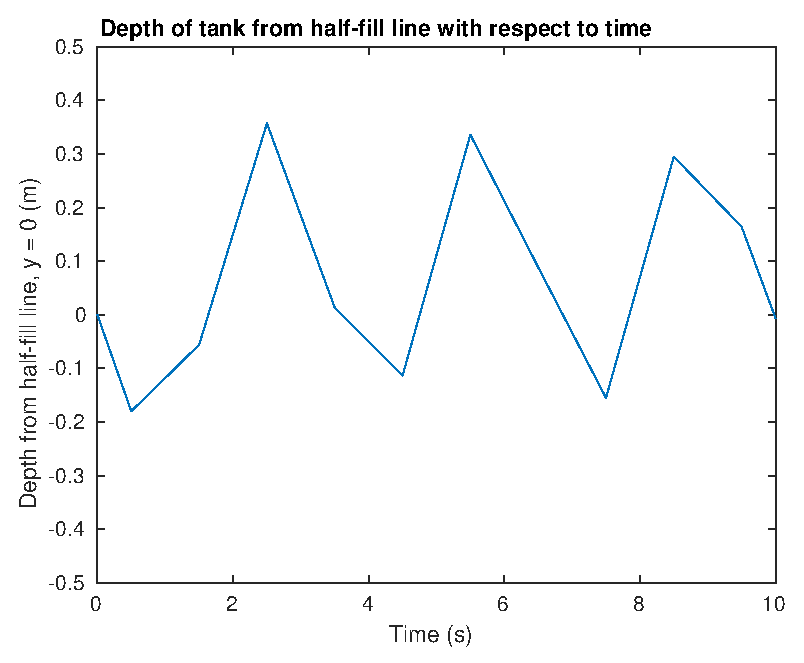
\includegraphics [width=4in]{cmcgarty_EE254_HW01_P1_9_01.eps}



\end{document}
    
